\documentclass[12pt]{report}
\usepackage[ngerman]{babel}            % German language support
\usepackage{amsmath, amssymb}          % Math support
\usepackage{graphicx}                  % Graphics support
\usepackage{lipsum}                    % For placeholder text (remove if not needed)
\usepackage{fancyhdr}                  % Custom headers/footers
\usepackage{datetime2}                 % Date formatting
\usepackage{float}                     % Figure placement
\usepackage{caption, subcaption}      % Captions for figures/tables
\usepackage{parskip}                   % Paragraph spacing
\usepackage{booktabs}                  % Professional tables
\usepackage[a4paper, width=160mm, top=25mm, bottom=25mm]{geometry} % Page layout
\usepackage{acronym}                   % Acronyms
\usepackage{tabularx}                  % Fixed-width tables
\usepackage[nottoc,notlot,notlof]{tocbibind} % Add bibliography to TOC
\usepackage{enumitem}                  % Custom lists
\usepackage{csquotes}                  % Quotation support
\usepackage{xcolor}
\usepackage{mdframed}
\usepackage[pdfa]{hyperref}                  % Hyperlinks (for PDF)
\usepackage{tikz}

% if hyperref does not work, use older version:
% sudo tlmgr install hyperref --version 7.01.06

% define environment for colored boxes
% Define custom colors
\definecolor{missionBlue}{RGB}{0, 102, 204}    % Professional blue
\definecolor{readyGreen}{RGB}{0, 153, 51}     % Ready/mission-ready green
\definecolor{alertRed}{RGB}{204, 0, 0}        % Alert/attention red
\definecolor{accentOrange}{RGB}{255, 102, 0}  % Highlight orange

\newcounter{equbox}
\newenvironment{equbox}[1][missionBlue]
  {\itshape
    \refstepcounter{equbox}\noindent%
   \begin{mdframed}[
       linewidth=1.5pt,
       roundcorner=5pt,
       innerleftmargin=10pt,
       innerrightmargin=10pt,
       linecolor=#1,            % Border color
       backgroundcolor=#1!10,   % Light background tint
       skipabove=\medskipamount,
       skipbelow=\medskipamount
   ]}
  {\end{mdframed}}

\newcounter{infobox}
\newenvironment{infobox}[1][readyGreen]
  {\itshape
    \refstepcounter{infobox}\noindent%
   \begin{mdframed}[
       linewidth=1.5pt,
       roundcorner=5pt,
       innerleftmargin=10pt,
       innerrightmargin=10pt,
       linecolor=#1,            % Border color
       backgroundcolor=#1!10,   % Light background tint
       skipabove=\medskipamount,
       skipbelow=\medskipamount
   ]}
  {\end{mdframed}}

\newcounter{bspbox}
\newenvironment{bspbox}
  {%
    \refstepcounter{bspbox}% Step the counter
    \medskip\noindent% Add vertical space and indent
    \itshape% Italic text for the content
    \textbf{Beispiel~\thebspbox:}\\% Title line
    \ignorespaces% Ignore extra spaces after \begin{bspbox}
  }
  {\par}% Add vertical space after the environment


% Graphics path
\graphicspath{{images/}}

% Hyperref setup
\hypersetup{
    colorlinks=false,                  % No colored links
    linktoc=all,                      % Link TOC entries
}

% Header and footer
\fancyhead[RO]{Marco Schnidrig}
\fancyhead[LO]{Physik - Grundlagen für MT HF 3. Semester}
% \fancyfoot[RO]{\thepage}
\fancyfoot[LO]{Kapitel \thechapter}
\renewcommand{\headrulewidth}{0.4pt}   % Header rule
\renewcommand{\footrulewidth}{0.4pt}   % Footer rule
\setlength{\headheight}{14.49998pt}    % Header height
\setlength{\parindent}{0em}            % No paragraph indent

% Document metadata
\newcommand{\docAuthor}{Marco Schnidrig}
\title{Physik - Grundlagen für MT HF  3. Semester\\ {\large Inovatech, Höhere Fachschule für Technik, Energie und Wirtschaft}}
\author{Marco Schnidrig}
\date{\today}

\begin{document}
	\maketitle 

	\tableofcontents
	\pagebreak

	\pagestyle{fancy}				% use from now on pagestyles (headers and footers...)

	%_____________________________________________________________________________________________________________________
	
	\chapter{Einleitung}
    
Physik ist die Grundlage für das Verständnis technischer Systeme im Maschinenbau und in der Systemtechnik.

Dieses Skript dient als zentrales Medium für den Physikunterricht im 3. Semester für Maschinentechniker Stufe HF an der Inovatech. 
Aufbauend auf den Grundkenntnissen der Mathematik und dem Physikskript von Semester 2 \cite{schnidrig_physik_2026}
vermittelt es die wichtigsten physikalischen Prinzipien, 
die für die Entwicklung und Optimierung moderner Technologien essenziell sind. Von Statik über Dynamik bis hin zur 
Strömungslehre werden die Inhalte möglichst anschaulich und praxisnah aufbereitet.

Wo auch immer möglich werden Beispiele und Aufgaben an reellen physikalischen Systemen gezeigt.
Diese sind meist stark vereinfacht und viele Einflüsse werden vernachlässigt, allerdings ist dies die 
Kunst für alle Stufen der Physik. Die Realität ist beliebig komplex, 
wer sie verständlich und isoliert vereinfachen kann, hat einen grossen Vorteil.

Nutzen Sie dieses Skript als Leitfaden, 
um den Einstieg in die Physik zu meistern und Ihre technischen Fähigkeiten zu vertiefen. 
Die behandelten Themen bieten eine solide Basis, die Sie je nach Interesse und Bedarf 
selbstständig vertiefen können. Literatur ist für alle Themengebiete im Überfluss erhältlich. 
Ziel des Unterrichts ist es, Ihnen die wichtigsten Werkzeuge 
an die Hand zu geben, um sich in neue Themengebiete einzuarbeiten und diese erfolgreich anzuwenden.

\begin{figure}[H]    
    \centering          %     left botm right top
    
\includegraphics[clip, trim=0cm 0cm 0cm 0cm,width=.3\textwidth]{physics_logo.jpg}
    \label{fig:einleitungPhysicsLogo}
\end{figure}

\newpage

\section{Organisation Unterricht}

Der Unterricht wird über OpenOlat organisiert. Der Unterricht ist als einfache Version des 
Flipped-Classrooms aufgebaut. Auf OpenOlat wird pro Unterrichtsblock ein Themenbereich oder Teile eines
Themenbereichs zugewiesen. Dieser ist vor dem jeweiligen Unterrichtsblock vorzubereiten.

In der ersten Lektion des Unterrichtblocks wird in einem kurzen Wrap-up der vorbereitete Stoff wiederholt.
Anschliessend werden allfällige Fragen beantwortet, der Rest des Unterrichts wird für das Lösen von Aufgaben genutzt.

Das Skript kann sich während des Semesters ändern, bitte achten Sie deshalb darauf, dass Sie auf
OpenOlat jeweils die aktuellste Version benutzen.

\section{Zu dem Skript}

Das Skript ist in die Themenbereiche aufgeteilt:

\begin{itemize}
    \item Statik 2
    \item Kinematik 2
    \item Hydrostatik
    \item Kontinuität und Bernoulli
    \item Schwingungen und Wellen 2
\end{itemize}

Zu jedem Themenbereich sind Übungen und Lösungen in den Anhängen \ref{app:A_Übungen} und \ref{app:B_Lösungen} abgelegt.

Das Skript basiert auf vielen verschiedenen Quellen, welche falls möglich referenziert werden.

Das Skript wird von der Lehrperson geschrieben und auf dem aktuellsten Stand gehalten.
Selbstverständlich sind Fehler vorhanden, falls Sie einen bemerken, wird ein Hinweis darauf
dankend entgegengenommen.
	\newpage

	\chapter{Statik 2}

Dieses Kapitel baut auf den folgenden Abschnitten im Skript des 2. Semesters \cite{schnidrig_physik_2026}:

\begin{minipage}[t]{.38\textwidth}
    \begin{itemize}
        \item Kraft
        \begin{itemize}
            \item Die resultierende Kraft
        \end{itemize}
        \item Moment
        \begin{itemize}
            \item Das Kräftepaar
            \item Schwerpunkt
        \end{itemize}
    \end{itemize}
\end{minipage}
\hspace{.1\textwidth}
\begin{minipage}[t]{.45\textwidth}
    \begin{itemize}
        \item Gleichgewicht eines Systems
        \begin{itemize}
            \item Zentrales Kräftesystem
            \item Parallele Kräfte
            \item Allgemeines Kräftesystem
        \end{itemize}
        \item Lagerung und Freimachen
        \begin{itemize}
            \item Das Freimachen
            \item Lagerungsarten
        \end{itemize}
    \end{itemize}
\end{minipage}

\begin{infobox}
    In der Statik - als Teilgebiet der Mechanik - wird von ruhenden und unverformbaren
    (starren) Körpern ausgegangen.
\end{infobox}

Ziel der Statik ist die Annahme der Lasten an einem
Bauteil, die Bestimmung von Lagerreaktionen und Schnittgrössen. Die Einteilung der Mechanik 
und der Statik ist in Abbildung \ref{fig:übersichtMechanikStatik} gezeigt.

\begin{figure}[H]    
    \centering          %     left botm right top
    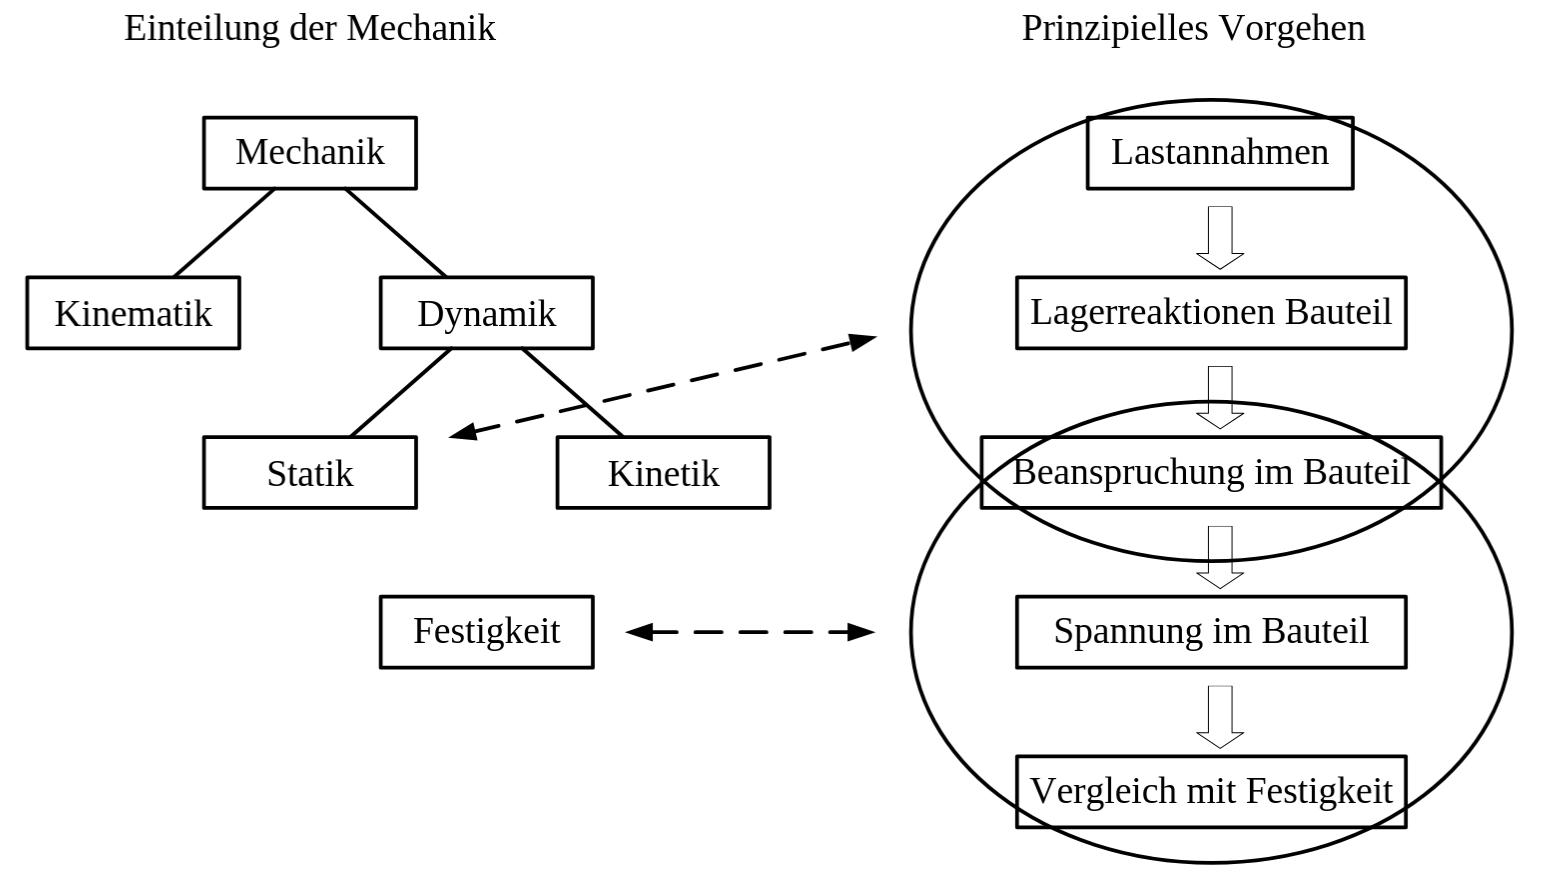
\includegraphics[clip, trim=0cm 0cm 0cm 0cm,width=.8\textwidth]{übersichtMechanikStatik.png} %.6 stands for 0.6 x textwidth
    \caption{Einteilung Mechanik und Statik}
    \label{fig:übersichtMechanikStatik}
\end{figure}

\section{Gleichgewicht für das ebene Kräftesystem}

Ein Bauteil ist dann im Gleichgewicht, wenn sich alle an ihm angreifenden Kräfte und
Momente gegenseitig aufheben. Für das freigemachte Bauteil heisst das, dass die
resultierende Kraft und das resultierende Moment verschwinden \cite{bartsch_mechanik_2022}.

\begin{infobox}
    Ein Körper befindet sich im Gleichgewicht, wenn die Summe aller angreifenden Kräfte und
    Momente gleich Null ist.
\end{infobox}

\begin{minipage}[t]{.35\textwidth}
    \begin{equbox}
        \begin{align}
            \sum F_x &= 0 \\
            \sum F_y &= 0 \\
            \sum M &= 0
        \end{align}
    \end{equbox}
\end{minipage}
\hspace{.1\textwidth}
\begin{minipage}[t]{.55\textwidth}
    \begin{figure}[H]    
        \centering          %     left botm right top
        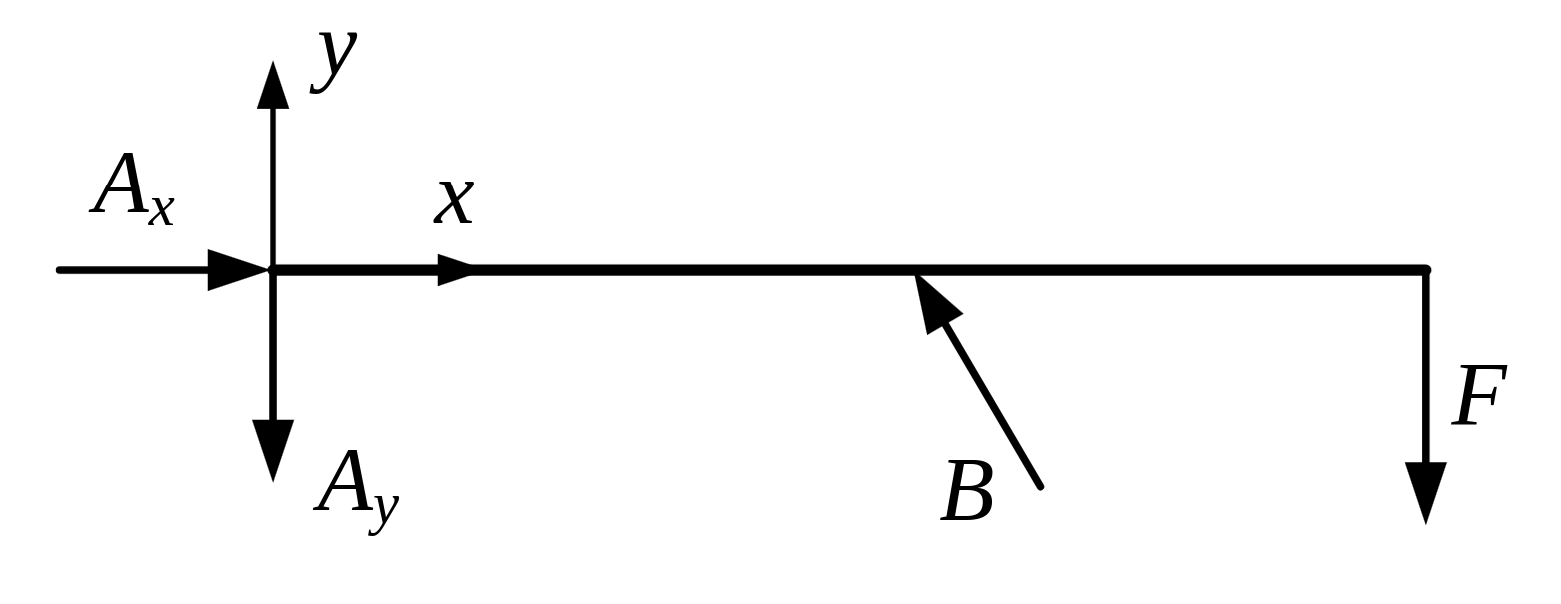
\includegraphics[clip, trim=0cm 0cm 0cm 0cm,width=.8\textwidth]{gleichgewicht_eines_systems.png} %.6 stands for 0.6 x textwidth
        \label{fig:gleichgewicht}
    \end{figure}
\end{minipage}

\begin{bspbox}
    Ein Generator mit Eigengewicht $G = 2000 N$ läuft mit einem Drehmoment von $M = 500 Nm$ im
    Uhrzeigersinn. Zusätzlich wirkt eine horizontale Kraft $F = 500 N$. Gesucht sind die Lagereaktionen in
    den Lagern $A$ und $B$.

    \begin{figure}[H]    
        \centering          %     left botm right top
        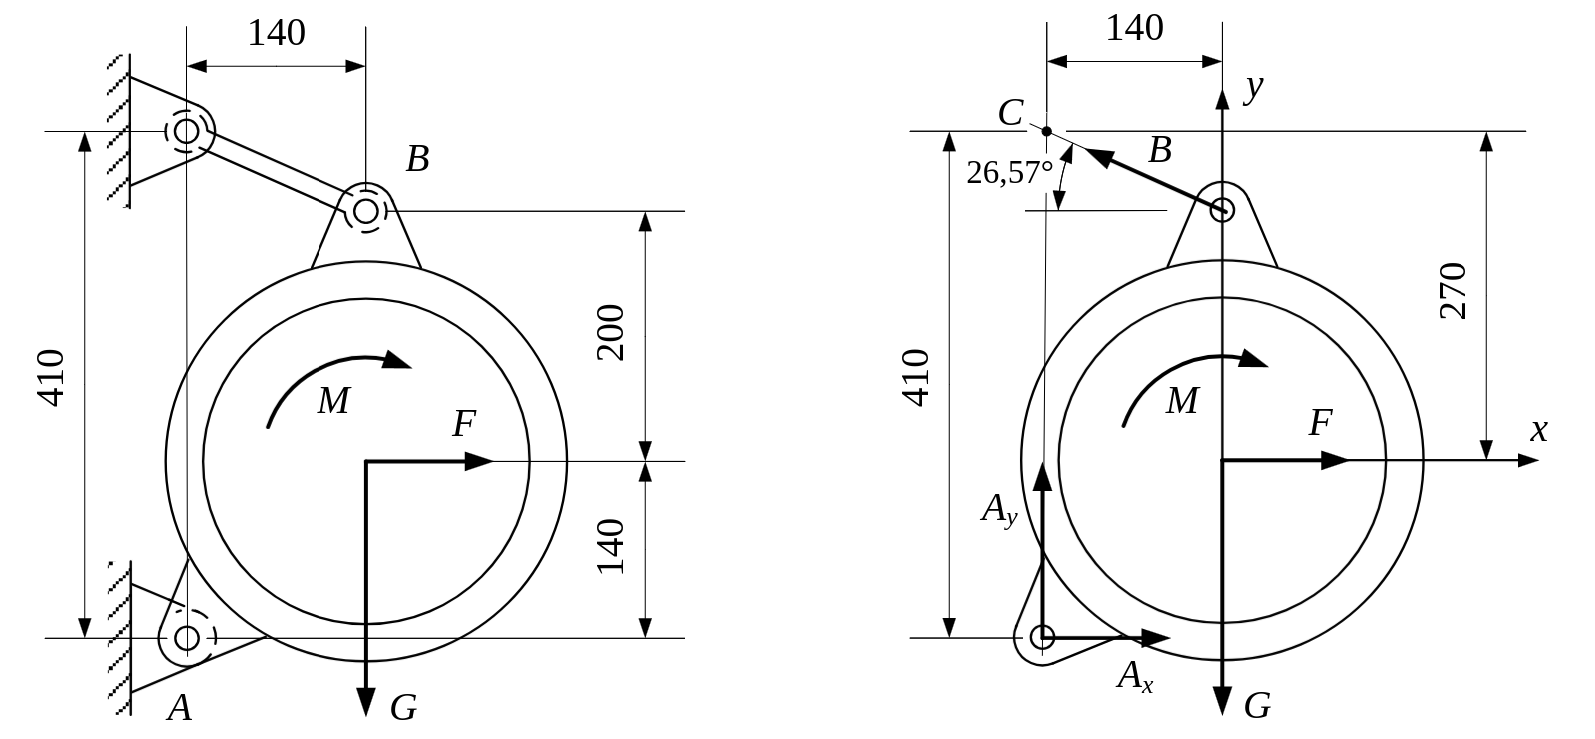
\includegraphics[clip, trim=0cm 0cm 0cm 0cm,width=.8\textwidth]{bsp_gleichgewicht.png} %.6 stands for 0.6 x textwidth
        \label{fig:bspgleichgewicht}
    \end{figure}

    Beim Aufstellen der 3 Gleichgewichtsbedingungen sind immer verschiedene Wege möglich. Mit einer
    Momentenbedingung bezüglich eines günstigen Pols kann man bereits eine Unbekannte bestimmen.
    Der Pol muss dabei nicht innerhalb des Bauteils sein. Hier wird der Punkt $C$ gewählt, durch welchen
    die beiden Kräfte $A_y$ und $B$ gehen.

    Die Wirkungslinie der Kraft $B$ ist durch die Verbindung der Punkte $B$ und $C$ gegeben (Pendelstütze).
    Der Winkel ergibt sich aus der Geometrie wie folgt:

    \begin{equation*}
        \tan^{-1}(\frac{70mm}{140mm}) = 26.57^{\circ}
    \end{equation*}

    \begin{align*}
        \sum M_C = 
    \end{align*}

\end{bspbox}

Das gezeigte Beispiel ist ein allgemeines Kräftesystem. 
Für die Spezialfälle fallen gegebenenfalls Gleichungen weg:

\begin{itemize}
    \item Zentrales Kräftesystem
    \begin{itemize}
        \item $\sum M = 0$ kann nicht aufgestellt werden
    \end{itemize}
    \item Parallele Kräftepaar
    \begin{itemize}
        \item $\sum F$ in eine Richtung wird nicht aufgestellt
    \end{itemize}
\end{itemize}

Ausserdem kann anstelle von $\sum F_x$ oder $\sum F_y$ eine weitere Momentengleichung $\sum M_{II}$ an 
einem anderen Punkt eingeführt werden.
	\newpage

	\chapter{Kinematik \& Dynamik 2}


	\newpage

	\chapter{Hydrostatik}
	\newpage

	\chapter{Schwingungen und Wellen 2}
	\newpage

	%_____________________________________________________________________________________________________________________

	\bibliographystyle{plainurl}
	\bibliography{PhysikInovatechSkripts}

	%_____________________________________________________________________________________________________________________
	
	\appendix 						% the following part will be appendix

	\chapter{Übungen}\label{app:A_Übungen}

\section{Einleitung}

\section{Statik 2}

\underline{Aufgabe 2.0.1}

\begin{minipage}{.58\textwidth}
    Drei Kräfte wirken auf den Körper.
    Das Mass $a$ ist $2m$.
    Zu bestimmen ist das Moment der Kräfte bezüglich
    dem Punkt $A$ sowie die Lagerkräfte $A_x$ und $A_y$.
    $F_1 = F_2 = F_3 = 10N$ (8)
\end{minipage}
\hspace{.1\textwidth}
\begin{minipage}{.3\textwidth}
    \begin{figure}[H]   
        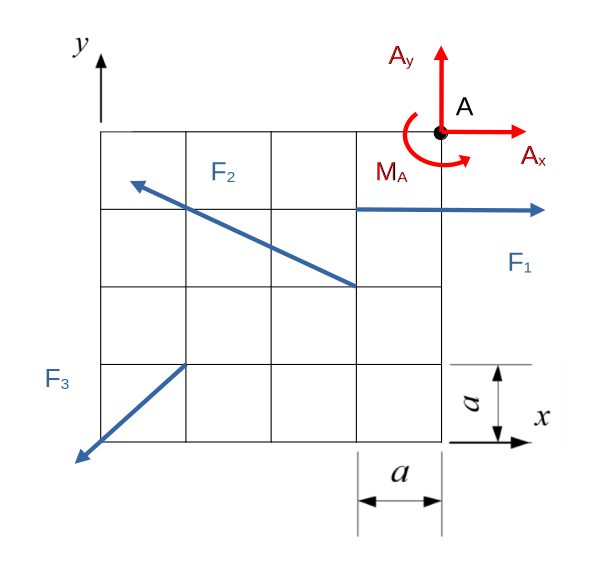
\includegraphics[width=\textwidth]{images/aufgabe_201.png} %.6 stands for 0.6 x textwidth
    \end{figure}
\end{minipage}

\underline{Aufgabe 2.0.2}

\begin{minipage}{.58\textwidth}
    An einem Hebel greifen 3 Kräfte an. \newline
    Es sind die auf die Welle 0 wirkende resultierende Kraft nach Betrag
    und Richtung und das resultierende Moment zu berechnen.
\end{minipage}
\hspace{.1\textwidth}
\begin{minipage}{.3\textwidth}
    \begin{figure}[H]    
        \centering          %     left botm right top
        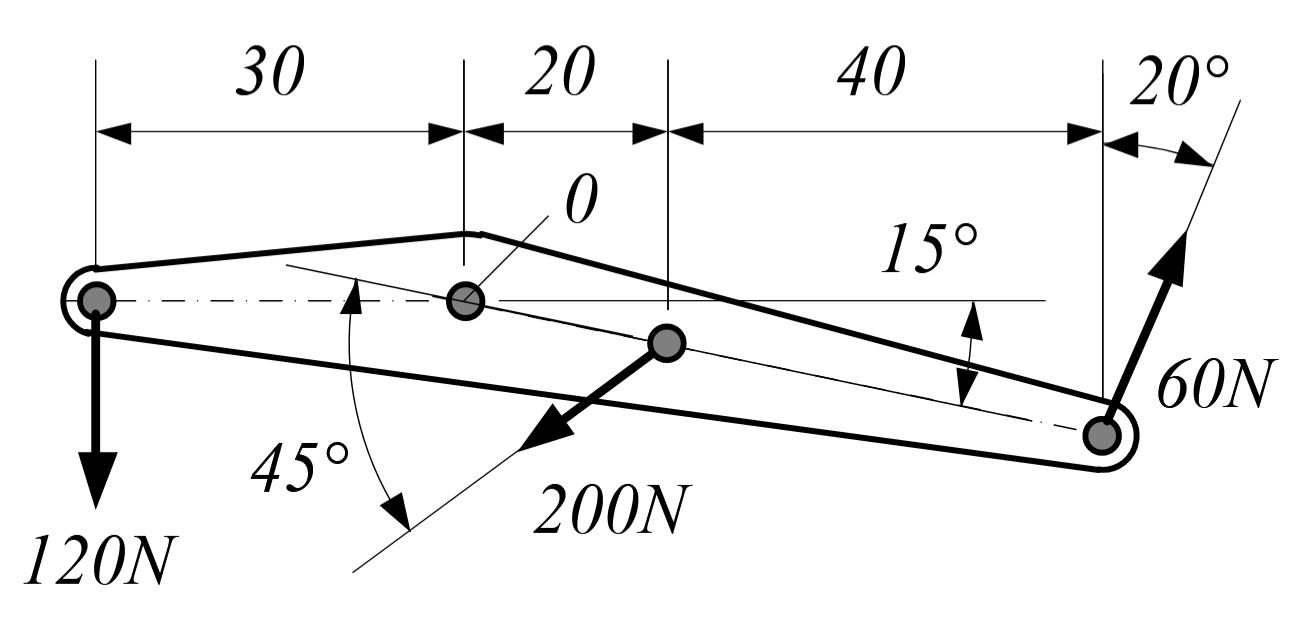
\includegraphics[clip, trim=0cm 0cm 0cm 0cm,width=\textwidth]{aufgabe_3_3_3_1.png} %.6 stands for 0.6 x textwidth
        \label{fig:3331}
    \end{figure}
\end{minipage}

\underline{Aufgabe 2.1.1}

\begin{minipage}{.58\textwidth}
    Ein Balken der Länge $l = 2m$ ist im Festlager $A$ (links) und im Loslager $B$
    (rechts) gelagert. Auf ihn wirken die vertikalen Kräfte $F = 300N$ im Abstand
    $0.5m$ von $A$ sowie $G = 100N$ in Balkenmitte. Am rechten Ende greift zusätzlich
    die horizontale Kraft $F_h = 50N$ an. \newline
    Zu bestimmen sind die Lagerreaktionen $A_x$, $A_y$ und $B$ sowie die
    dimensionierende Lagerkraft $A$.
\end{minipage}
\hspace{.05\textwidth}
\begin{minipage}{.35\textwidth}
    \begin{figure}[H]   
        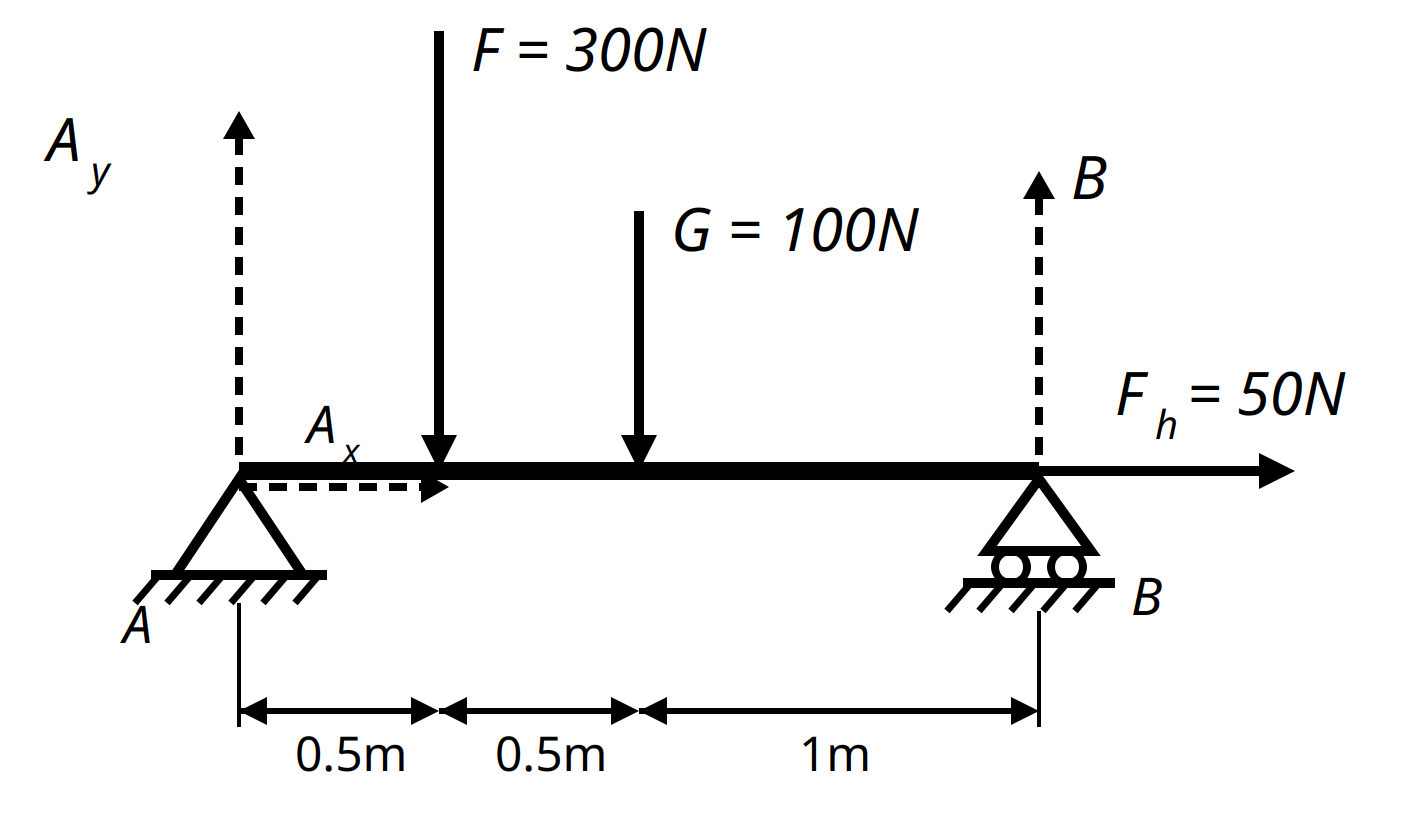
\includegraphics[width=\textwidth]{aufgabe_2_1_1.png}
    \end{figure}
\end{minipage}

\underline{Aufgabe 2.1.2}

\begin{minipage}{.58\textwidth}
    Zu bestimmen sind die Seilkraft und die 
    Auflagerreaktion in A.
\end{minipage}
\hspace{.1\textwidth}
\begin{minipage}{.3\textwidth}
    \centering
    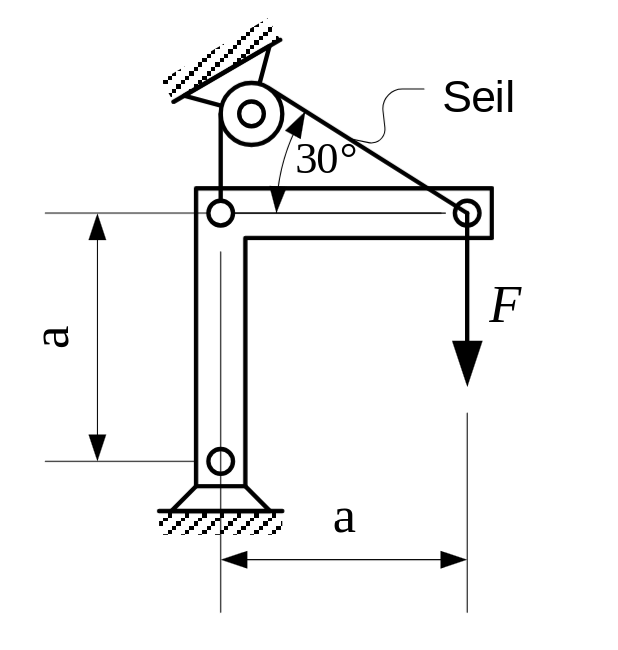
\includegraphics[width=\linewidth]{aufgabe_2_1_2.png}
\end{minipage}

	\chapter{Lösungen}\label{app:B_Lösungen}

\underline{2.0.1}:
$M_A = 24.72Nm, A_x = 6.015N, A_y = 2.599N$

\underline{2.0.2}:
$F_{res} = 223.8N, \alpha = 47^{\circ}, M_{res, 0} = 4385Nmm (\circlearrowleft)$

\underline{2.1.1}:
$B = 125N (\uparrow), A_y = 275N (\uparrow), A_x = -50N (\leftarrow), A = 279.5N$

\underline{2.1.2}: $S = 24.89kN$; $A_x = 21.56kN (\rightarrow)$;
$A_y = 3.33kN(\downarrow)$; $A = 21.8kN$

	\chapter{Tabellen}\label{app:C_tabellen}



\end{document}
